\documentclass{article}
\usepackage[letter, margin=0.95in]{geometry}
\usepackage{graphicx}  % for including images
\usepackage{listings}  % for code formatting
\usepackage{hyperref}  % for URLs

\title{Mini Project 1 Report: Web \& Proxy Server}
\author{Neel Sadafule and Dylan Cantafio}
\date{\today}

% Define lstlisting settings for better line breaks
\lstset{
    breaklines=true,  % Break long lines
    breakatwhitespace=true,  % Allow breaking at whitespace
    basicstyle=\ttfamily,  % Monospaced font
}

\begin{document}

\maketitle

\section*{Step One: Determine Requirements}

In this step, we implemented a simple web server capable of responding to different HTTP requests with the appropriate status codes as outlined by RFC 7231, Section 6. The web server is expected to handle the following status codes: \texttt{200 OK}, \texttt{304 Not Modified}, \texttt{400 Bad Request}, \texttt{404 Not Found}, and \texttt{501 Not Implemented}.

\subsection*{200 OK}

\begin{itemize}
    \item \textbf{Description}: This status code indicates that the request was successful, and the server is returning the requested resource.
    \item \textbf{Logic}: 
    The server generates \texttt{200 OK} when:
    \begin{itemize}
        \item The request uses the \texttt{GET} method.
        \item The request path points to an existing file (e.g., \texttt{test.html}).
        \item The HTTP version is valid (i.e., \texttt{HTTP/1.1}).
        \item The headers are properly formatted.
    \end{itemize}
    If these conditions are met, the server reads the requested file and sends its content along with the \texttt{200 OK} status code.
    \item \textbf{Request}: The following \texttt{curl} command was used to test the \texttt{200 OK} status:
\begin{lstlisting}
curl http://localhost:8080/test.html
\end{lstlisting}
    \item \textbf{Expected Output}: The contents of \texttt{test.html} should be displayed, and the response header should include \texttt{200 OK}.
\end{itemize}

\subsection*{304 Not Modified}

\begin{itemize}
    \item \textbf{Description}: This status code indicates that the requested resource has not been modified since the time specified in the \texttt{If-Modified-Since} header, and the server is not returning any content.
    \item \textbf{Logic}: 
    The server generates \texttt{304 Not Modified} when:
    \begin{itemize}
        \item The request uses the \texttt{GET} method.
        \item The \texttt{If-Modified-Since} header is present in the request.
        \item The last modification time of the requested file is earlier than or equal to the time specified in the \texttt{If-Modified-Since} header.
    \end{itemize}
    In this case, the server does not return the file contents but instead returns the \texttt{304 Not Modified} status code.
    \item \textbf{Request}: The following \texttt{curl} command was used to test the \texttt{304 Not Modified} status:
\begin{lstlisting}
curl -H "If-Modified-Since: Mon, 21 Oct 2024 13:27:34 GMT" http://localhost:8080/test.html
\end{lstlisting}
    \item \textbf{Expected Output}: The server will return a \texttt{304 Not Modified} status with no content.
\end{itemize}

\subsection*{400 Bad Request}

\begin{itemize}
    \item \textbf{Description}: This status code indicates that the server could not understand the request due to malformed syntax.
    \item \textbf{Logic}: 
    The server generates \texttt{400 Bad Request} when:
    \begin{itemize}
        \item The request is malformed or incomplete.
        \item Essential headers like \texttt{Host} are missing or incorrectly formatted.
        \item The request line does not follow the correct format (i.e., method, path, and HTTP version).
    \end{itemize}
    The server responds with this code when it cannot parse the request correctly.
    \item \textbf{Request}: The following \texttt{curl} command was used to test the \texttt{400 Bad Request} status:
\begin{lstlisting}
curl -H "Host:" http://localhost:8080/test.html
\end{lstlisting}
    \item \textbf{Expected Output}: The server will return a \texttt{400 Bad Request} status with an explanation of the error in the headers.
\end{itemize}

\subsection*{404 Not Found}

\begin{itemize}
    \item \textbf{Description}: This status code indicates that the requested resource could not be found on the server.
    \item \textbf{Logic}: 
    The server generates \texttt{404 Not Found} when:
    \begin{itemize}
        \item The requested file does not exist on the server.
        \item The client’s request path points to a non-existent file or directory.
    \end{itemize}
    If this condition is met, the server responds with the \texttt{404 Not Found} status code.
    \item \textbf{Request}: The following \texttt{curl} command was used to test the \texttt{404 Not Found} status:
\begin{lstlisting}
curl http://localhost:8080/nonexistent.html
\end{lstlisting}
    \item \textbf{Expected Output}: The server will return a \texttt{404 Not Found} status, indicating that the file does not exist.
\end{itemize}

\subsection*{501 Not Implemented}

\begin{itemize}
    \item \textbf{Description}: This status code indicates that the server does not support the requested method (e.g., \texttt{POST}, \texttt{PUT}).
    \item \textbf{Logic}: 
    The server generates \texttt{501 Not Implemented} when:
    \begin{itemize}
        \item The request uses an unsupported HTTP method such as \texttt{POST} or \texttt{PUT}.
    \end{itemize}
    The server only supports the \texttt{GET} method, and if any other method is used, it responds with the \texttt{501 Not Implemented} status code.
    \item \textbf{Request}: The following \texttt{curl} command was used to test the \texttt{501 Not Implemented} status:
\begin{lstlisting}
curl -X POST http://localhost:8080/test.html
\end{lstlisting}
    \item \textbf{Expected Output}: The server will return a \texttt{501 Not Implemented} status, indicating that the \texttt{POST} method is not supported.
\end{itemize}


\section*{Step Two: Build Minimal Web Server \& Test}

In this step, we built a minimal web server using socket programming and the HTTP protocol. The server listens for incoming HTTP requests and processes them, responding with the appropriate HTTP status codes as implemented in Step One. No Python HTTP libraries were used to ensure compliance with the project requirements.

\subsection*{Web Server Implementation}

We implemented a basic web server that listens on port 8080 for incoming HTTP requests. The server parses incoming requests, determines the appropriate response based on the logic described in Step One, and returns the requested file or status code. The HTML file \texttt{test.html} was placed in the main directory to test the correct working scenario.

\subsubsection*{Server Behavior and Request Handling}
The server follows a request-response model as per the HTTP protocol:
\begin{itemize}
    \item Listens for incoming connections on a known port (8080 in this case).
    \item Parses the incoming HTTP request, including method, path, and headers.
    \item Responds with the appropriate status code and content based on the request and the logic implemented in Step One.
\end{itemize}

\subsection*{Server Startup and Browser Test}

\begin{itemize}
    \item \textbf{Starting the Server}:
    We started the server by running the following command in the terminal:
    \begin{lstlisting}
    python3 web_server.py
    \end{lstlisting}
    The server successfully started and began listening for incoming connections on port 8080.

    \item \textbf{IP Address Test}:
    We used \texttt{localhost} as the IP address and port 8080 to access the server. The web server can be tested in the browser by typing the following URL:
    \begin{quote}
        \texttt{http://localhost:8080/test.html}
    \end{quote}
    This returned the contents of \texttt{test.html}, confirming that the server was correctly serving the file.

    \item \textbf{Screenshot of Server Running}:
    \begin{center}
        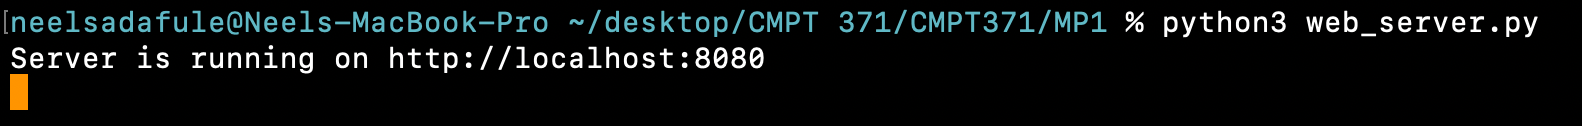
\includegraphics[width=\textwidth]{screenshots/server_start.png}  
    \end{center}

    \item \textbf{Browser Access Test}: 
    The contents of \texttt{test.html} were accessed through a web browser at the URL:
    \begin{quote}
        \texttt{http://localhost:8080/test.html}
    \end{quote}
    The server correctly returned the contents of \texttt{test.html}, confirming that the server was working as expected.

    \item \textbf{Screenshot of Browser Test}:
    \begin{center}
        
\includegraphics[width=\textwidth]{screenshots/browser_test.png}  % Replace with the actual screenshot path
    \end{center}
\end{itemize}

\subsection*{Status Code Testing Using \texttt{curl}}

The following tests were conducted using \texttt{curl} commands to verify that the server returns the correct status codes as described in Step One.

\subsubsection*{200 OK}
\begin{itemize}
    \item \textbf{Test Command}:
    \begin{lstlisting}
    curl -i http://localhost:8080/test.html
    \end{lstlisting}
    \item \textbf{Screenshot of Terminal Output}:
    \begin{center}
        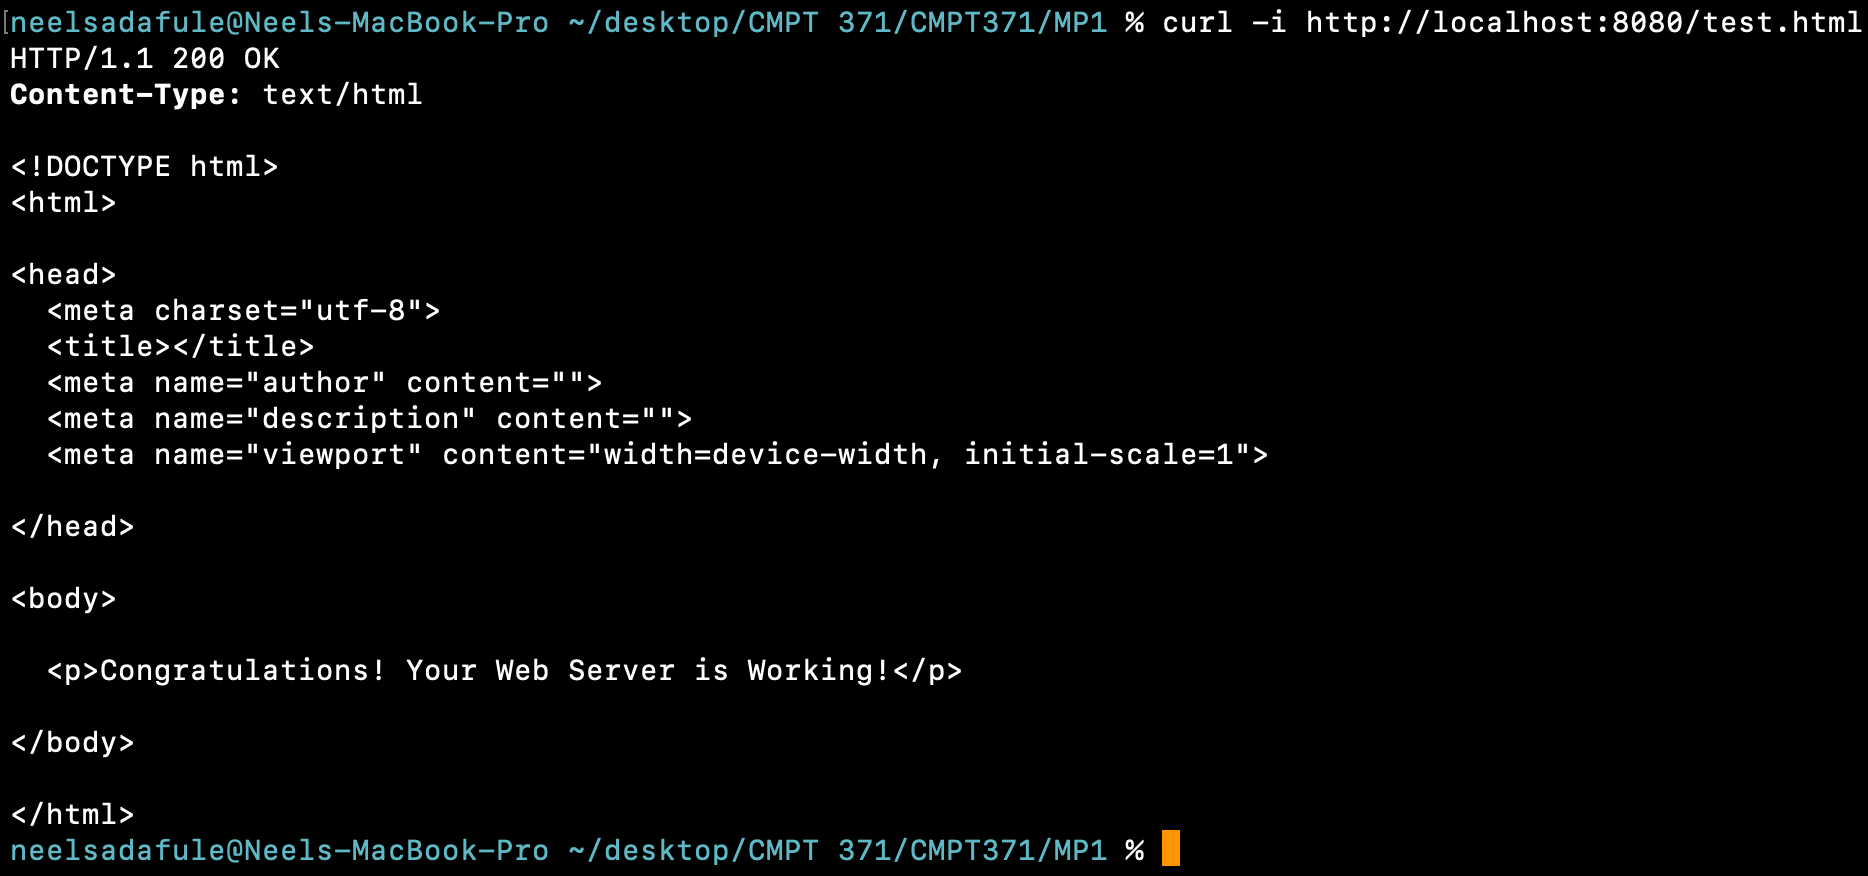
\includegraphics[width=\textwidth]{screenshots/200_OK.png}
    \end{center}
\end{itemize}

\subsubsection*{304 Not Modified - Detailed Case}

We conducted two separate tests for the \texttt{304 Not Modified} status: one where the file \texttt{test.html} was not modified, and one where it was modified after the \texttt{If-Modified-Since} header.

\subsubsection*{Checking Last Modified Time of \texttt{test.html}}

Before conducting the tests, we checked the last modified time of \texttt{test.html} using the following command:
\begin{lstlisting}
stat -f "%Sm" test.html
\end{lstlisting}
The output showed the current modification time.

\begin{center}
    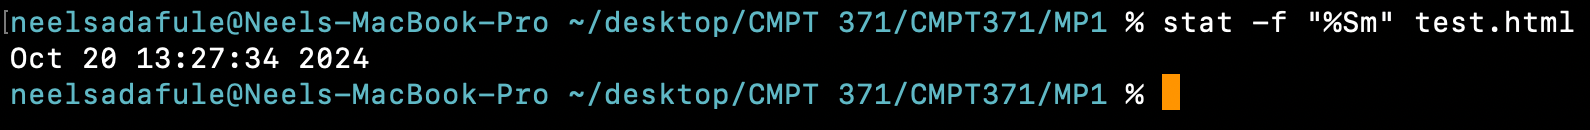
\includegraphics[width=\textwidth]{screenshots/check_last_modified.png}  % Replace with actual screenshot path
\end{center}

\subsubsection*{Case 1: \texttt{test.html} Not Modified}

\begin{itemize}
    \item \textbf{Test Command}: We ran the following command to simulate a request with the \texttt{If-Modified-Since} header.
    \begin{lstlisting}
    curl -i -H "If-Modified-Since: Mon, 21 Oct 2024 13:27:34 GMT" http://localhost:8080/test.html
    \end{lstlisting}

    \item \textbf{Expected Outcome}: The server returned \texttt{304 Not Modified} because \texttt{test.html} had not been modified since the specified date. The output did not contain any content, as expected. According to the HTTP/1.1 specification, the response contains only the status code and headers.

    \item \textbf{Screenshot of Terminal Output}:
    \begin{center}
        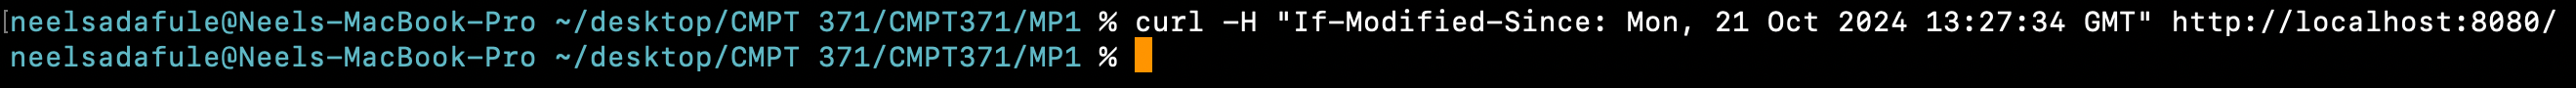
\includegraphics[width=\textwidth]{screenshots/304_Not_Modified.png}  % Replace with actual screenshot path
    \end{center}
\end{itemize}

\subsubsection*{Case 2: \texttt{test.html} Modified}

We modified the contents of \texttt{test.html} by adding text to the file, and then we checked its last modified time using the same command:
\begin{lstlisting}
stat -f "%Sm" test.html
\end{lstlisting}
The output showed the updated modification time.

\begin{center}
    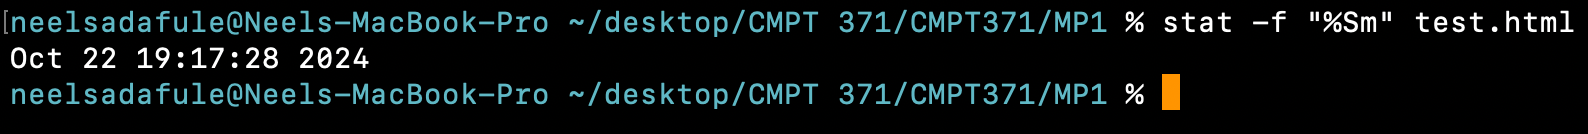
\includegraphics[width=\textwidth]{screenshots/check_modified.png}  % Replace with actual screenshot path
\end{center}

\begin{itemize}
    \item \textbf{Test Command}: We ran the same \texttt{curl} command with the \texttt{If-Modified-Since} header:
    \begin{lstlisting}
    curl -H "If-Modified-Since: Mon, 21 Oct 2024 13:27:34 GMT" http://localhost:8080/test.html
    \end{lstlisting}

    \item \textbf{Expected Outcome}: The server returned \texttt{200 OK} along with the contents of \texttt{test.html}, since the file had been modified after the specified date.

    \item \textbf{Screenshot of Terminal Output}:
    \begin{center}
        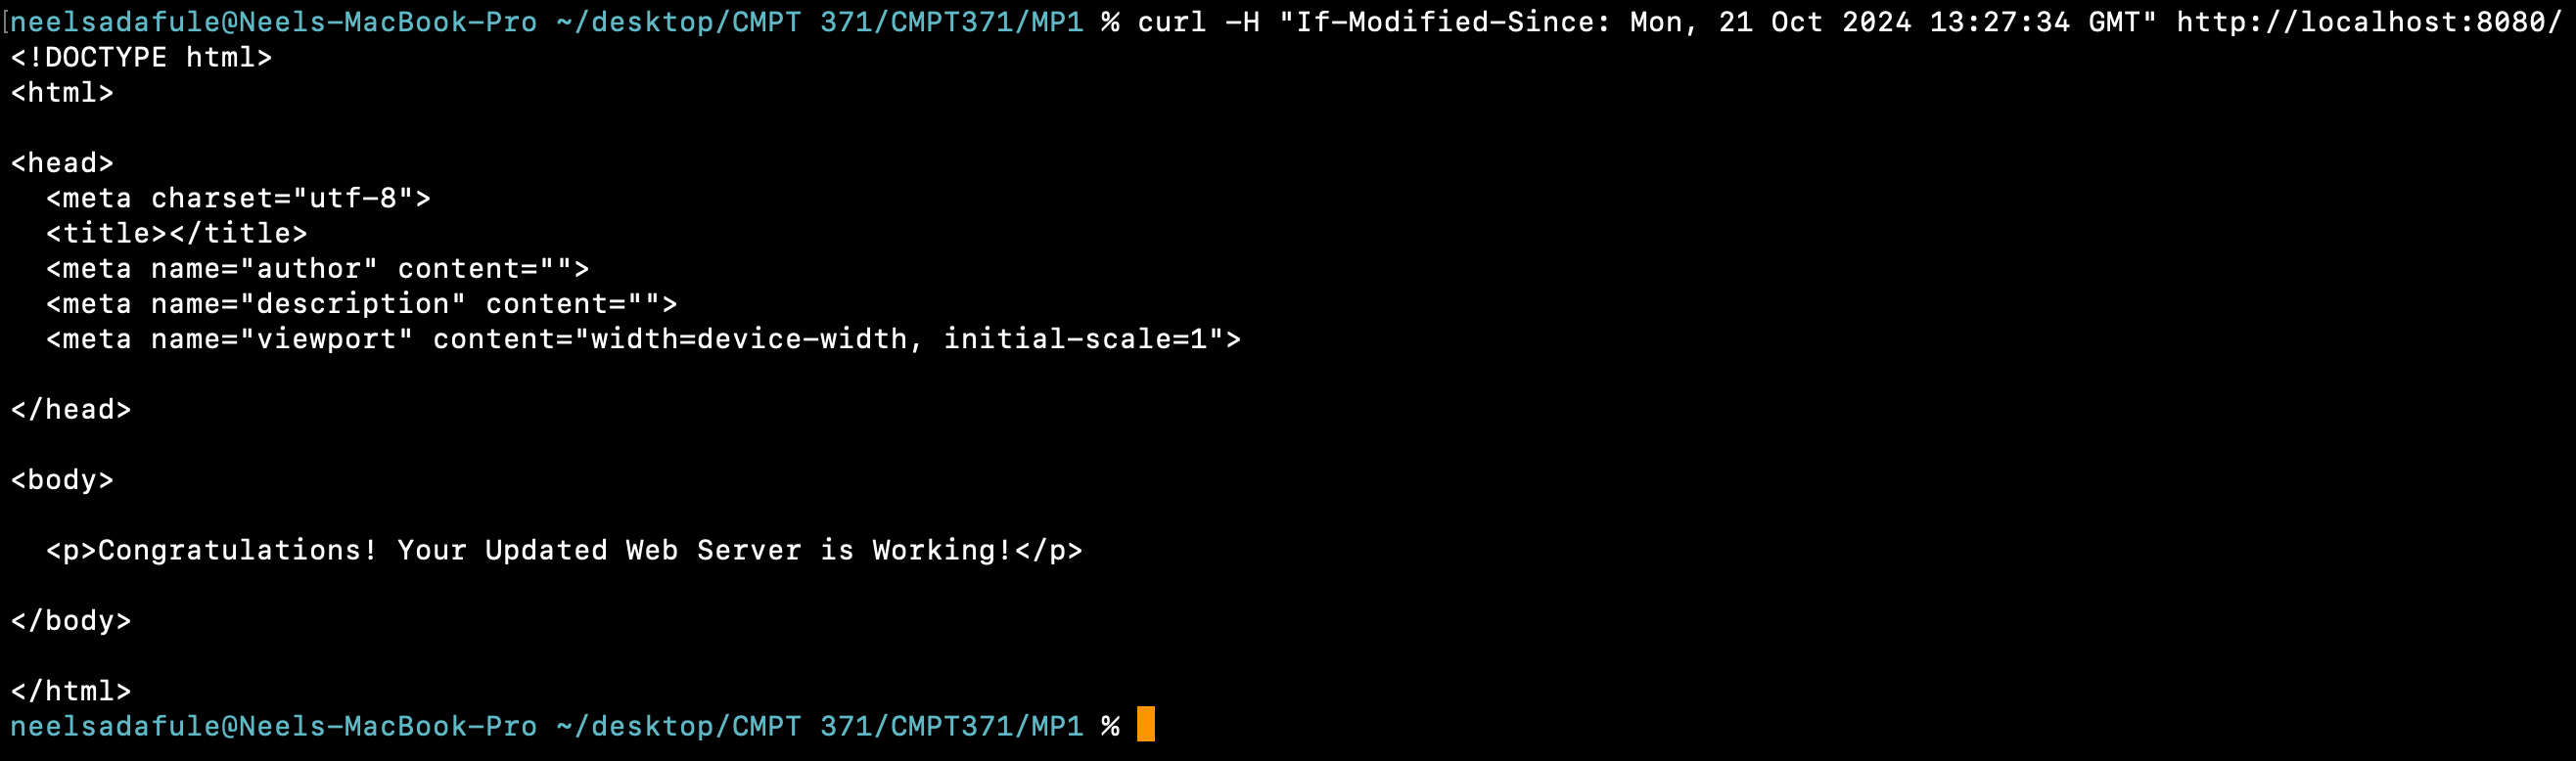
\includegraphics[width=\textwidth]{screenshots/200_OK_after_modification.png}  % Replace with actual screenshot path
    \end{center}
\end{itemize}

\subsubsection*{400 Bad Request}
\begin{itemize}
    \item \textbf{Test Command}:
    \begin{lstlisting}
    curl -i -H "Host:" http://localhost:8080/test.html
    \end{lstlisting}

    \item \textbf{Test Output}: The server returned \texttt{400 Bad Request} because the request was malformed (specifically, the \texttt{Host} header was missing or incorrectly formatted).

    \item \textbf{Screenshot of Terminal Output}:
    \begin{center}
        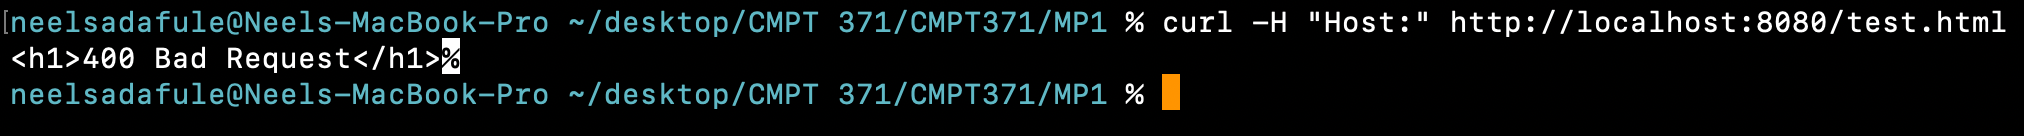
\includegraphics[width=\textwidth]{screenshots/400_Bad_Request.png}  % Replace with the actual screenshot path
    \end{center}
\end{itemize}

\subsubsection*{404 Not Found}
\begin{itemize}
    \item \textbf{Test Command}:
    \begin{lstlisting}
    curl -i http://localhost:8080/nonexistent.html
    \end{lstlisting}

    \item \textbf{Test Output}: The server returned \texttt{404 Not Found} because the requested file did not exist.

    \item \textbf{Screenshot of Terminal Output}:
    \begin{center}
        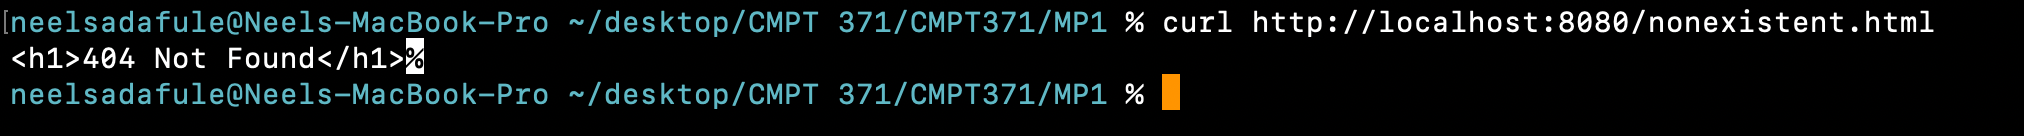
\includegraphics[width=\textwidth]{screenshots/404_Not_Found.png}  % Replace with the actual screenshot path
    \end{center}
\end{itemize}

\subsubsection*{501 Not Implemented}
\begin{itemize}
    \item \textbf{Test Command}:
    \begin{lstlisting}
    curl -i -X POST http://localhost:8080/test.html
    \end{lstlisting}

    \item \textbf{Test Output}: The server returned \texttt{501 Not Implemented} because the \texttt{POST} method is not supported by the server, which only supports \texttt{GET}.

    \item \textbf{Screenshot of Terminal Output}:
    \begin{center}
        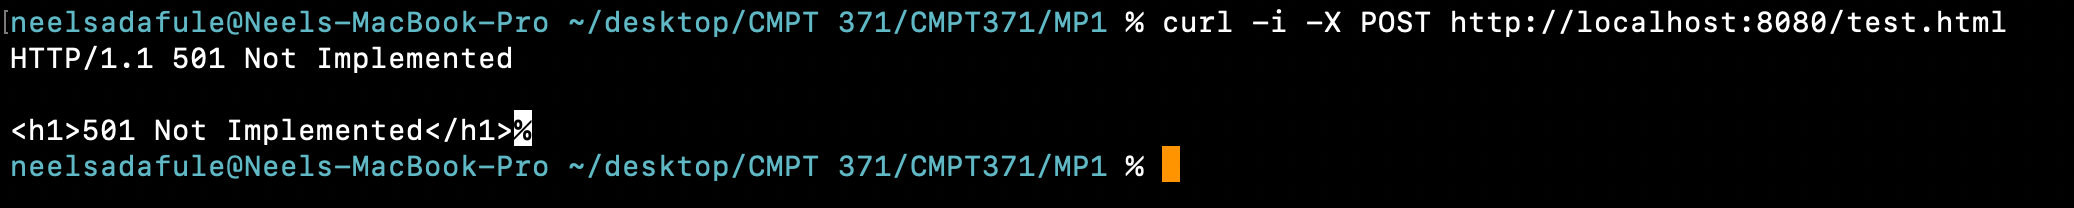
\includegraphics[width=\textwidth]{screenshots/501_Not_Implemented.png}  % Replace with the actual screenshot path
    \end{center}
\end{itemize}

\section*{Step Three: Performance}

This section evaluates the performance of the Proxy Server and the Multi-threaded Web Server. Each subsection describes the server's specifications, the procedure to start it, and the tests performed with corresponding screenshots.

\subsubsection*{Difference Between Proxy Server and Web Server}

A proxy server differs from a standard web server in that it acts as an intermediary between a client and an external server. While a web server serves files from its local filesystem, a proxy server forwards client requests to another server (e.g., \texttt{httpbin.org}) and relays the response back to the client. Proxy servers can also provide additional functionality like caching, load balancing, and access control.

\subsection*{Proxy Server}

\subsubsection*{Proxy Server Specifications}

In this implementation, the proxy server forwards client requests to an external server (\texttt{httpbin.org}) and relays the response back to the client. It listens on port 8888 and handles requests concurrently.

\begin{itemize}
    \item \textbf{Request Handling}: The proxy server forwards client requests to \texttt{httpbin.org} and sends back the response to the client.
    \item \textbf{Concurrency}: Each client request is handled in a separate thread.
\end{itemize}

\subsubsection*{Proxy Server Start Procedure}

\begin{itemize}
    \item Start the proxy server by running the following command:
    \begin{lstlisting}
    python3 proxy_server.py
    \end{lstlisting}
    \item Screenshot of the terminal showing the proxy server running.
    \begin{center}
        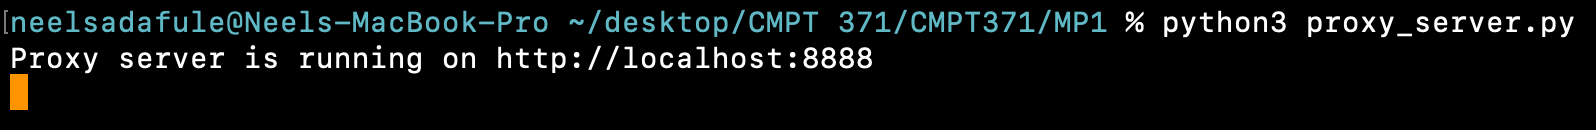
\includegraphics[width=\textwidth]{screenshots/proxy_server_start.png}  % Replace with actual screenshot
    \end{center}
\end{itemize}

\subsubsection*{Proxy Server Testing}

We tested the proxy server by sending a request using \texttt{curl}. The server forwarded the request to \texttt{httpbin.org} and returned the response.

\begin{itemize}
    \item Test the proxy server by running the following command:
    \begin{lstlisting}
    curl http://localhost:8888/get
    \end{lstlisting}
    \item Expected Outcome: The proxy server forwards the request to \texttt{httpbin.org}, and the response includes request headers and origin information in JSON format.
    \item Screenshot of the terminal output:
    \begin{center}
        \includegraphics[width=\textwidth]{screenshots/proxy_server_test.png}  % Replace with actual screenshot
    \end{center}
\end{itemize}

\subsection*{Multi-threaded Web Server}

\subsubsection*{Why Multi-threaded Web Server and Impact on Performance}

In a single-threaded web server, the server processes one request at a time, which means other incoming requests must wait until the current one is complete. This can result in significant delays, particularly if one request takes a long time to process (e.g., due to file I/O or network latency). By switching to a multi-threaded model, the web server can handle multiple requests concurrently. Each request is processed in a separate thread, allowing the server to respond to clients in parallel and improving overall responsiveness and throughput.

\subsubsection*{Multi-threaded Web Server Specifications}
In this implementation, each incoming request spawns a new thread, allowing the server to serve multiple clients simultaneously. This improves performance, especially under heavy loads, and reduces client wait times. It listens on port 8080 and serves local files, such as \texttt{test.html}.

\begin{itemize}
    \item \textbf{Request Handling}: The web server responds to requests by serving local files, like \texttt{test.html}.
    \item \textbf{Concurrency}: The server spawns a new thread for each incoming request, allowing concurrent file access.
\end{itemize}

\subsubsection*{Multi-threaded Web Server Start Procedure}

\begin{itemize}
    \item Start the web server by running the following command:
    \begin{lstlisting}
    python3 web_server.py
    \end{lstlisting}
    \item Screenshot of the terminal showing the web server running.
    \begin{center}
        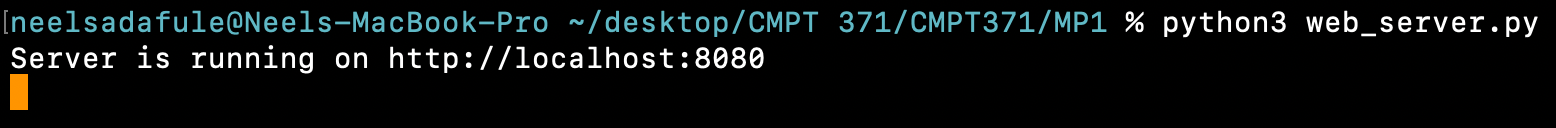
\includegraphics[width=\textwidth]{screenshots/web_server_start.png}  % Replace with actual screenshot
    \end{center}
\end{itemize}

\subsubsection*{Multi-threaded Web Server Testing}

We tested the web server by sending concurrent requests using the following commands in the same terminal:

\begin{itemize}
    \item Test the server by running the following commands:
    \begin{lstlisting}
    curl http://localhost:8080/test.html &
    curl http://localhost:8080/test.html &
    curl http://localhost:8080/test.html &
    \end{lstlisting}
    \item Expected Outcome: The server responds to all requests concurrently by serving the contents of \texttt{test.html}.
    \item Screenshot of the terminal output:
    \begin{center}
        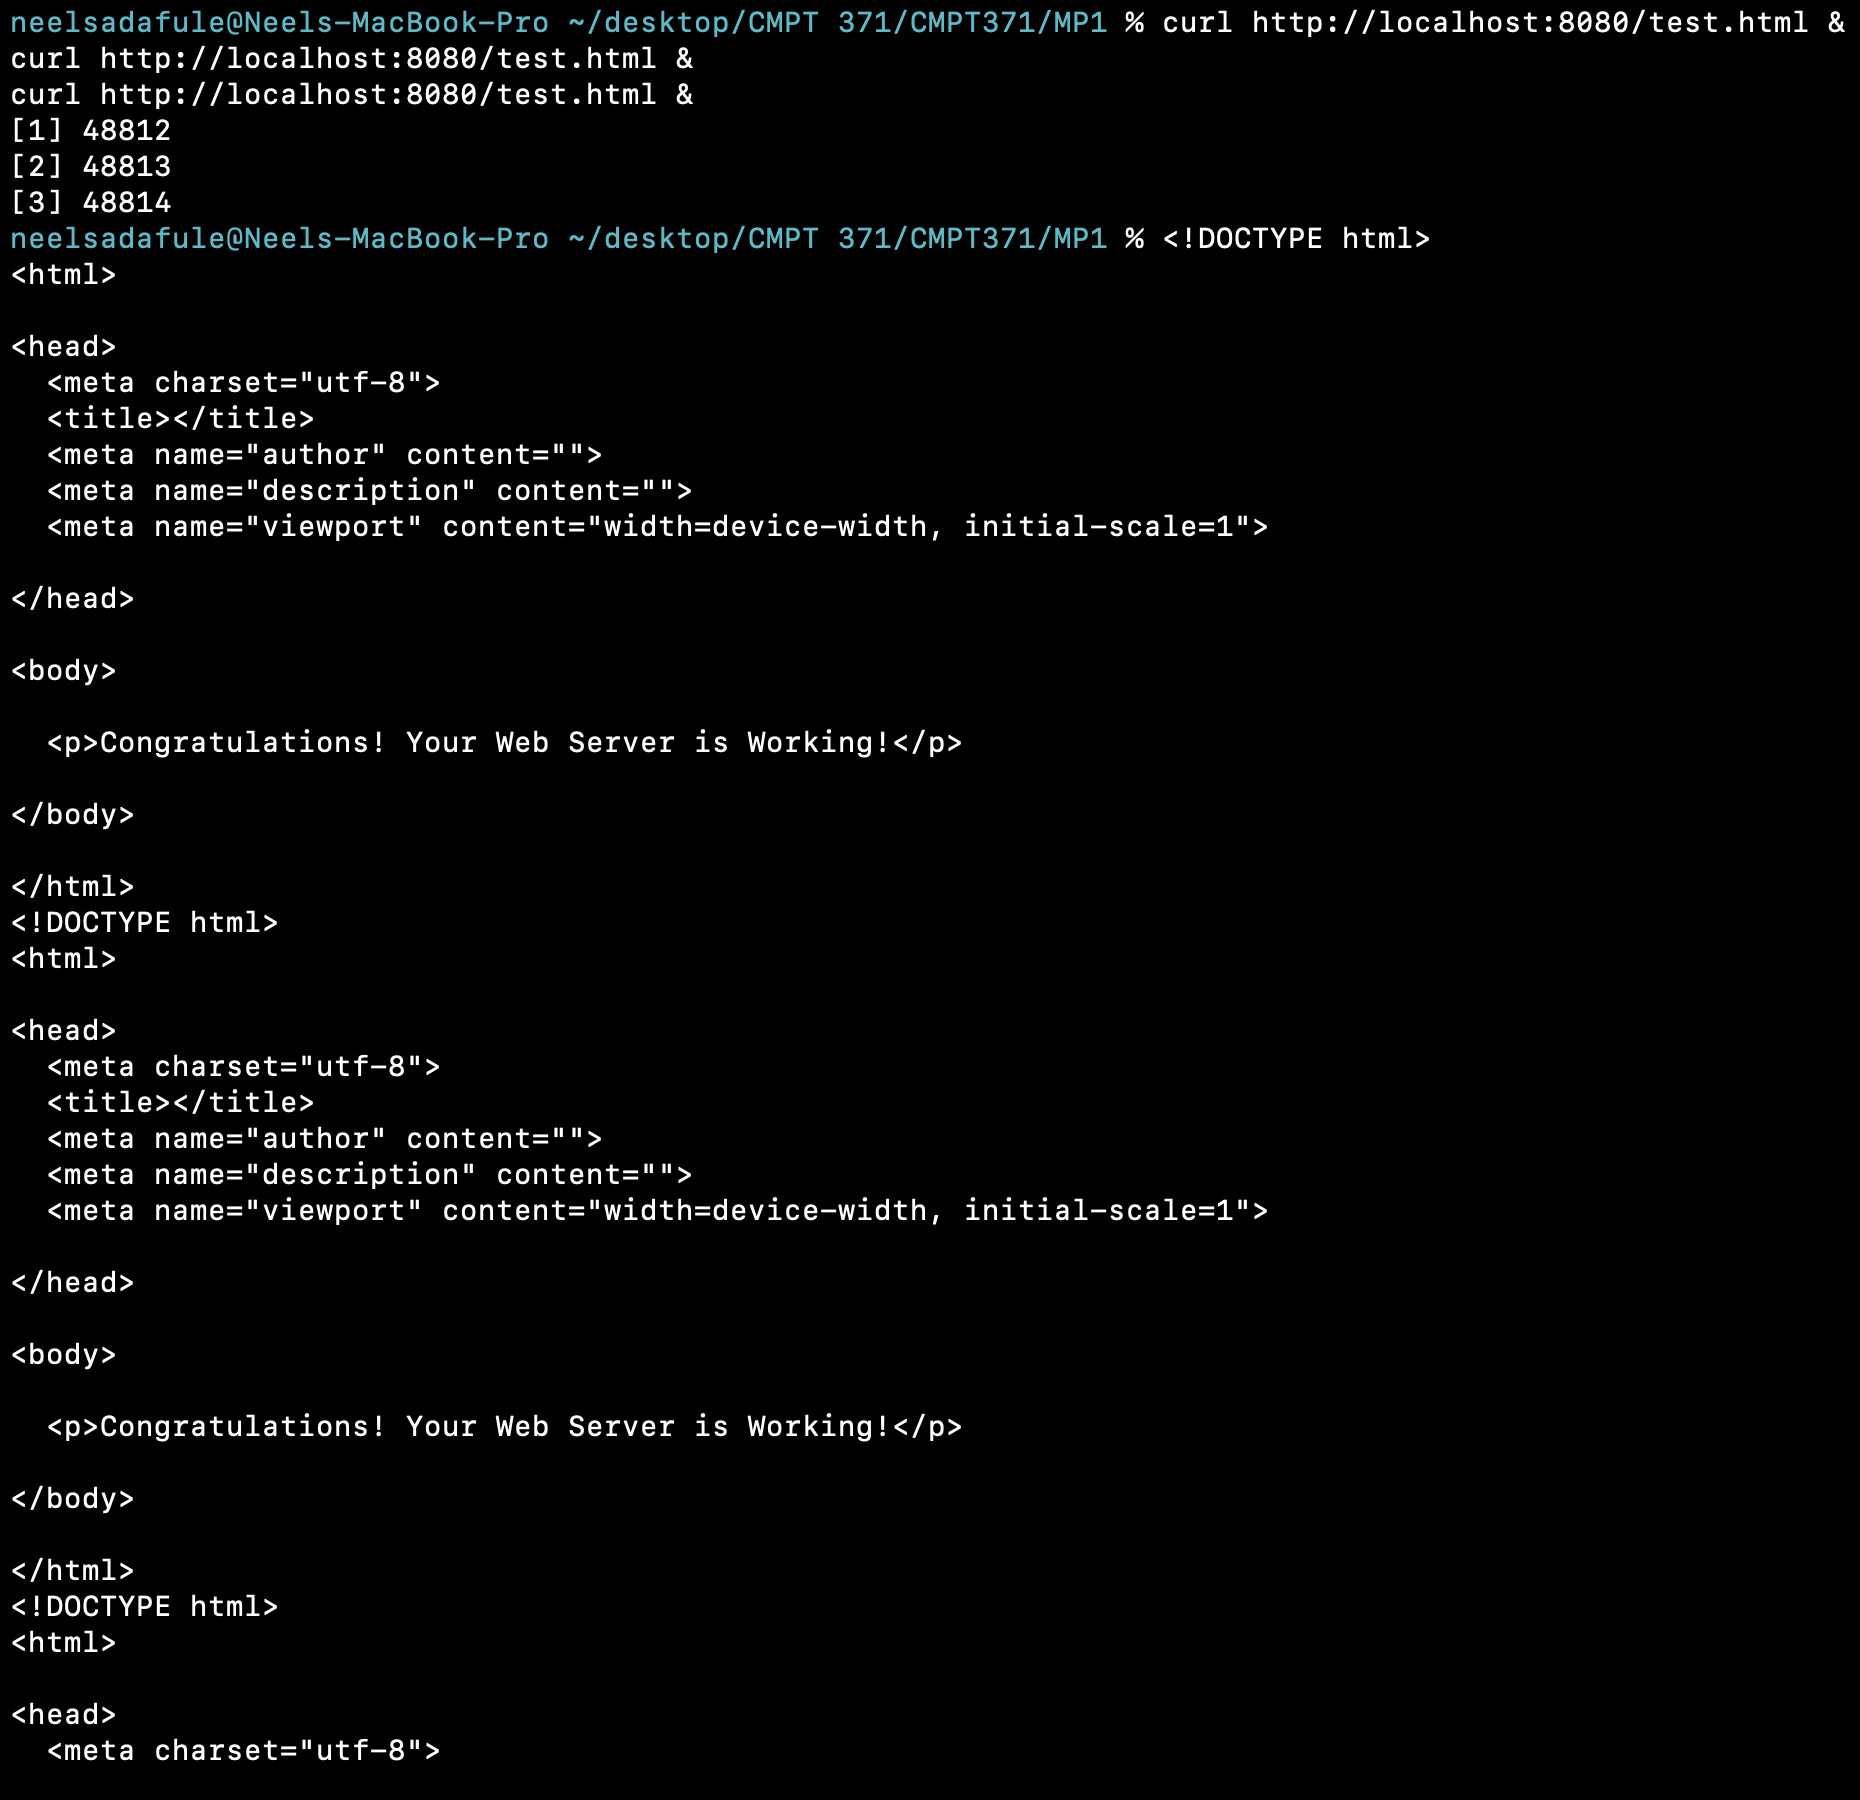
\includegraphics[width=\textwidth]{screenshots/multithreaded_test1.png}  % Replace with actual screenshot
    \end{center}
    \begin{center}
        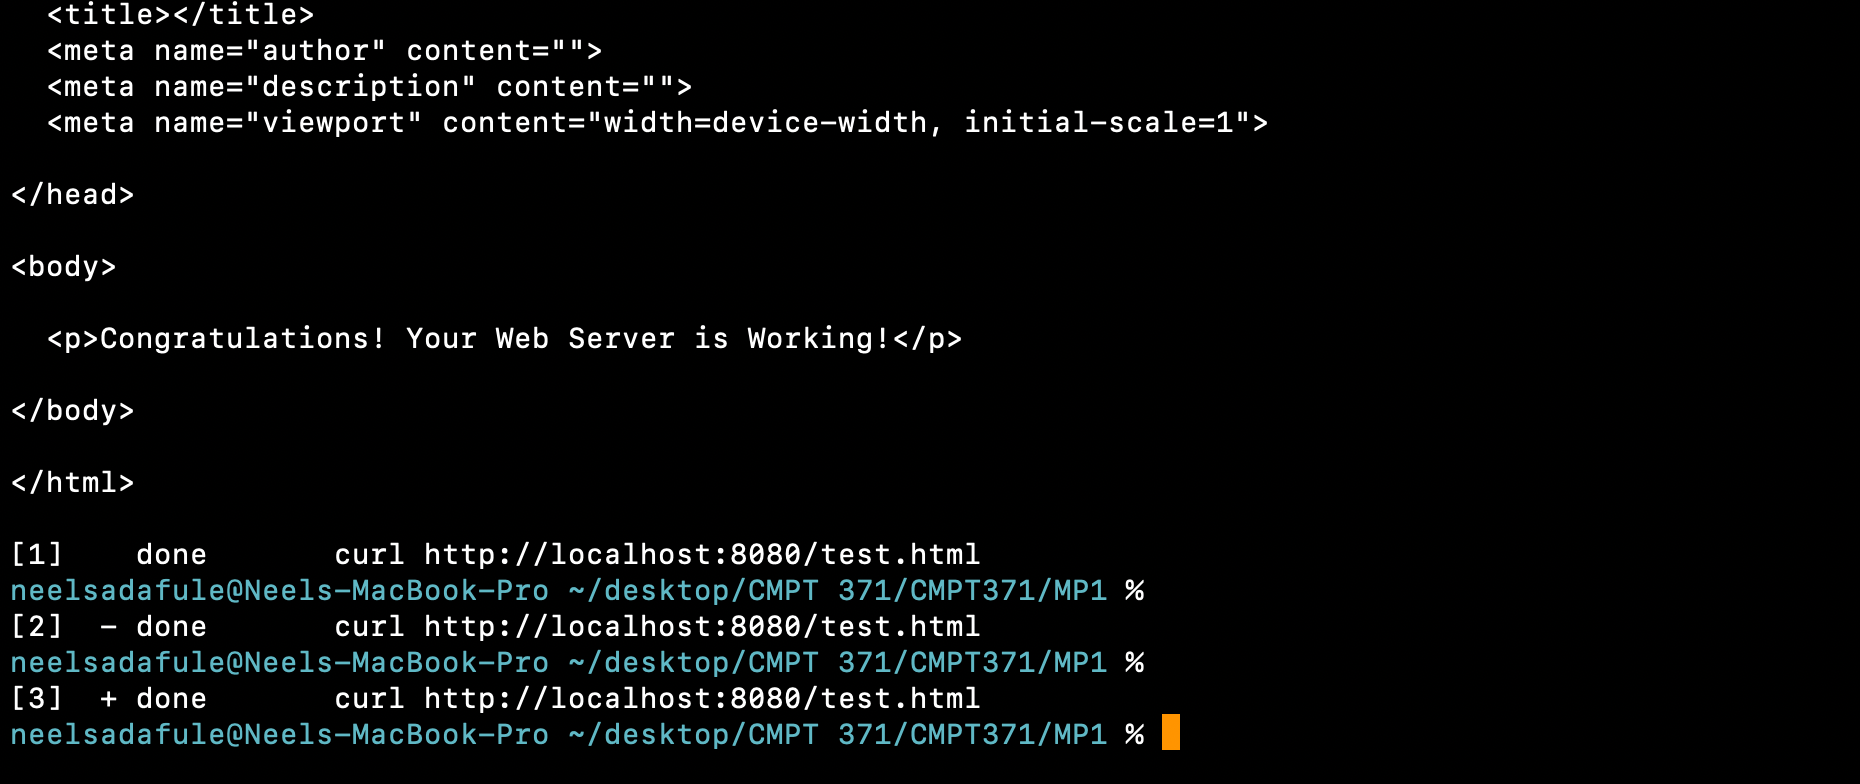
\includegraphics[width=\textwidth]{screenshots/multithreaded_test2.png}  % Replace with actual screenshot
    \end{center}
\end{itemize}

\section*{Step Four: Expand}

In this step, we addressed the Head-of-Line (HOL) blocking problem in the multi-threaded web server \texttt{web\_server.py}. HOL blocking occurs when a large or slow request prevents other requests from being processed, which can significantly impact performance. To avoid this issue, we implemented a simulated frame-based approach similar to HTTP/2.

\subsection*{Avoiding HOL Blocking with Frames}

HOL Blocking problem can significantly degrade performance, especially in a multi-client environment. We modified the server to process and send responses in smaller chunks (frames) rather than sending the entire content in a single transmission. Each request receives its data incrementally, without waiting for other requests to finish. This allows the server to serve multiple requests concurrently without one request blocking others. Additionally, we introduced a small delay between frames to simulate a more realistic network environment.

\begin{itemize}
    \item \textbf{Frame-based Response}: We split the response content into 1KB chunks and sent each chunk separately. This simulates how HTTP/2 interleaves multiple responses in small frames, avoiding the HOL blocking issue.
    \item \textbf{Concurrency}: Since the server is multi-threaded, it can handle multiple requests simultaneously. Each request's response is interleaved with the others, improving overall performance and reducing wait times for smaller requests.
\end{itemize}

\subsection*{Testing HOL Blocking Avoidance}

To test the impact of our changes, we sent concurrent requests to the server using the following commands:
\begin{itemize}
    \item Test the server by running the following commands:
    \begin{lstlisting}
    curl http://localhost:8080/test.html &
    curl http://localhost:8080/test.html &
    curl http://localhost:8080/test.html &
    \end{lstlisting}
    \item Expected Outcome: The server responds to all requests concurrently by serving the contents of \texttt{test.html}.
    \item Screenshot of the terminal output:
    \begin{center}
        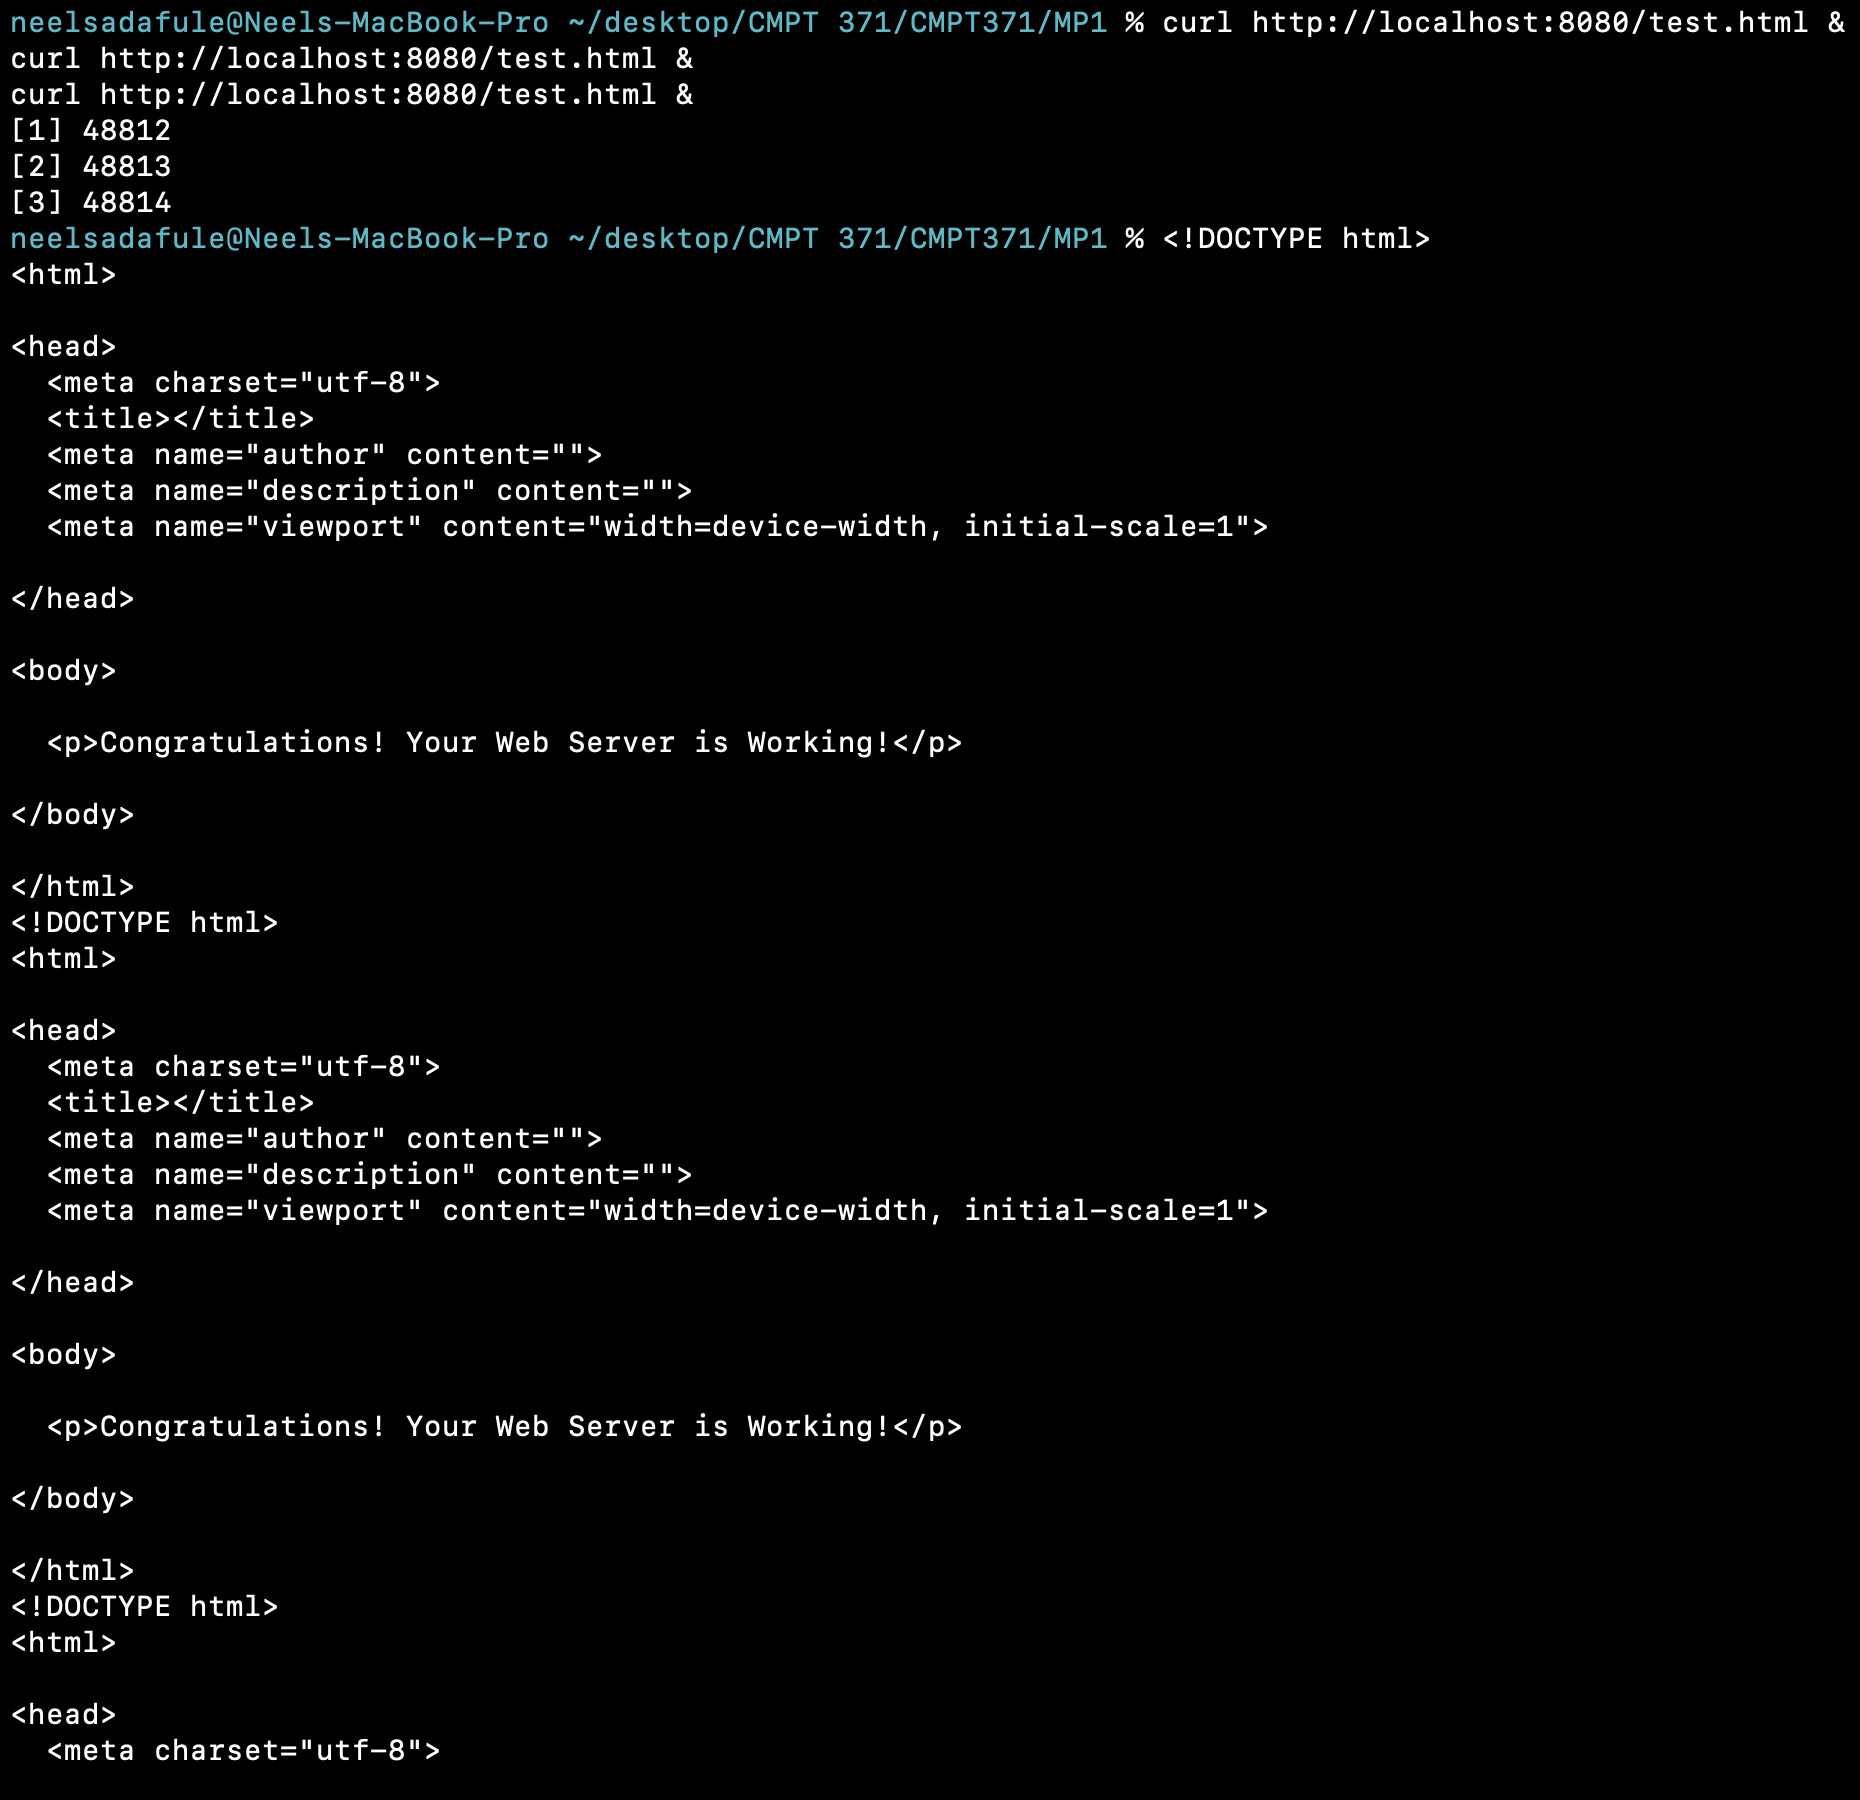
\includegraphics[width=\textwidth]{screenshots/multithreaded_test1.png}  % Replace with actual screenshot
    \end{center}
    \begin{center}
        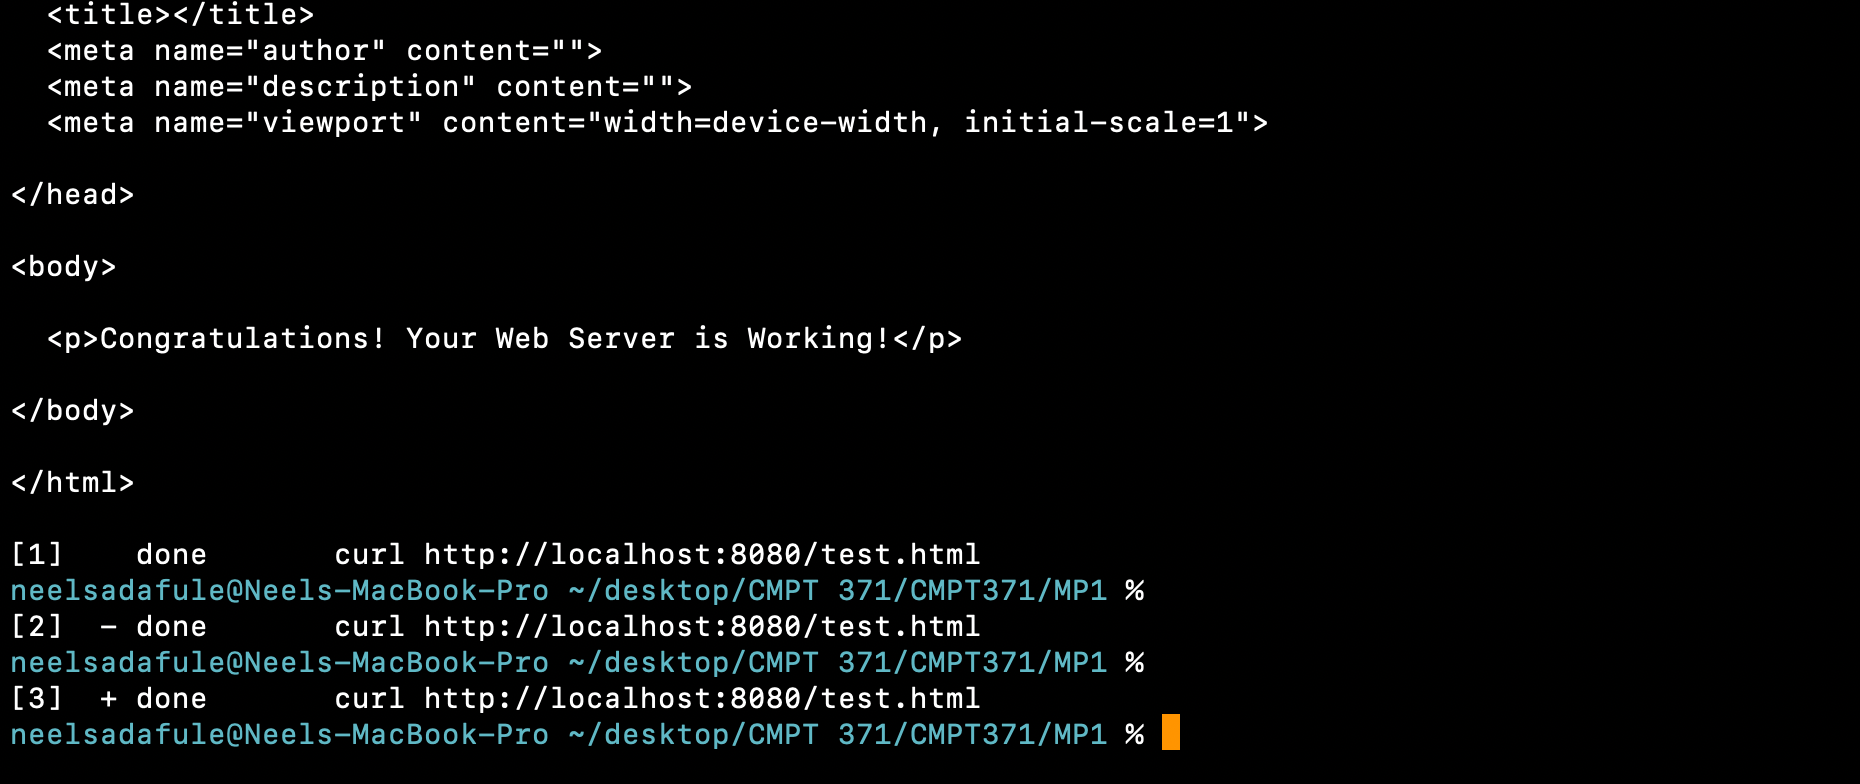
\includegraphics[width=\textwidth]{screenshots/multithreaded_test2.png}  % Replace with actual screenshot
    \end{center}
\end{itemize}

The server successfully processed multiple requests concurrently, and the frame-based response ensured that no single request blocked the others, effectively avoiding HOL blocking.

\subsection*{Testing HOL Blocking with Concurrent Requests}

We further tested the HOL blocking avoidance by running a large number of concurrent requests using a loop to simulate multiple clients accessing the server at once. The server should handle all requests without blocking and serve the content chunk-by-chunk.

\subsubsection*{Test Procedure}

We used the following looped `curl` command to generate 50 concurrent requests:
\begin{lstlisting}
for i in {1..50}; do curl http://localhost:8080/test.html & done
\end{lstlisting}

\subsubsection*{Expected Outcome}

The server should be able to process all 50 requests concurrently, serving the content chunk-by-chunk without experiencing HOL blocking. Each request should receive a portion of the content without waiting for any other request to complete.

\subsubsection*{Screenshot of Test Output}

\begin{itemize}
    \item \textbf{Client Terminal}: The terminal will show multiple concurrent `curl` commands being executed.
    \begin{center}
    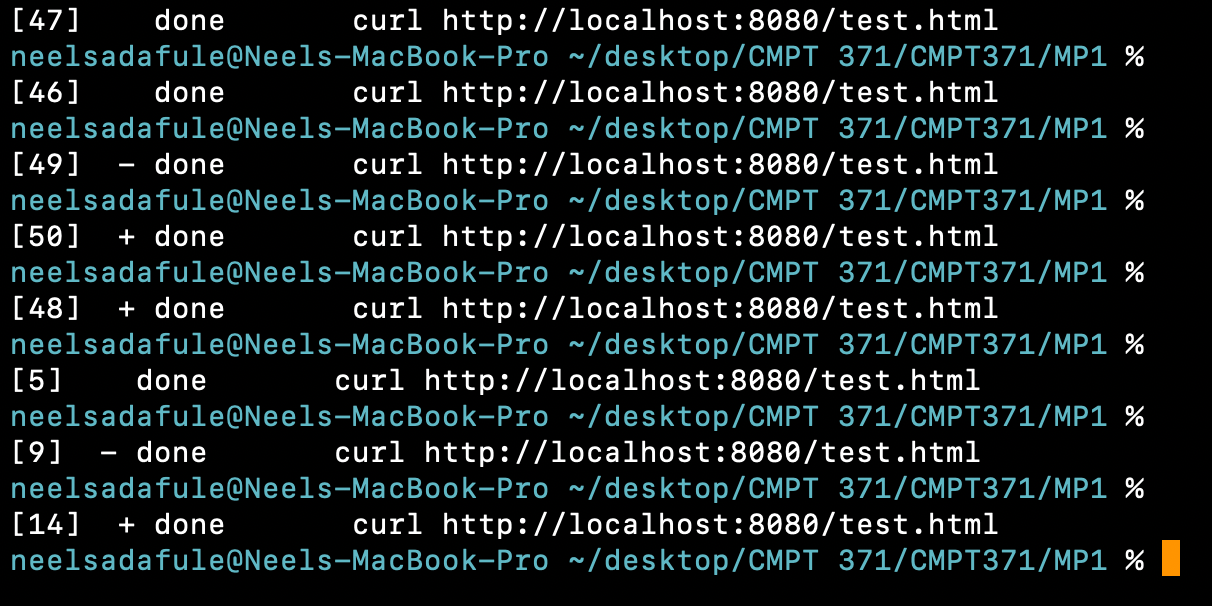
\includegraphics[width=\textwidth]{screenshots/hol_blocking_loop_test_client.png}  % Replace with actual client screenshot
    \end{center}
    \item \textbf{Server Terminal}: The terminal will display logs for each connection as it handles multiple requests in parallel.
    \begin{center}
    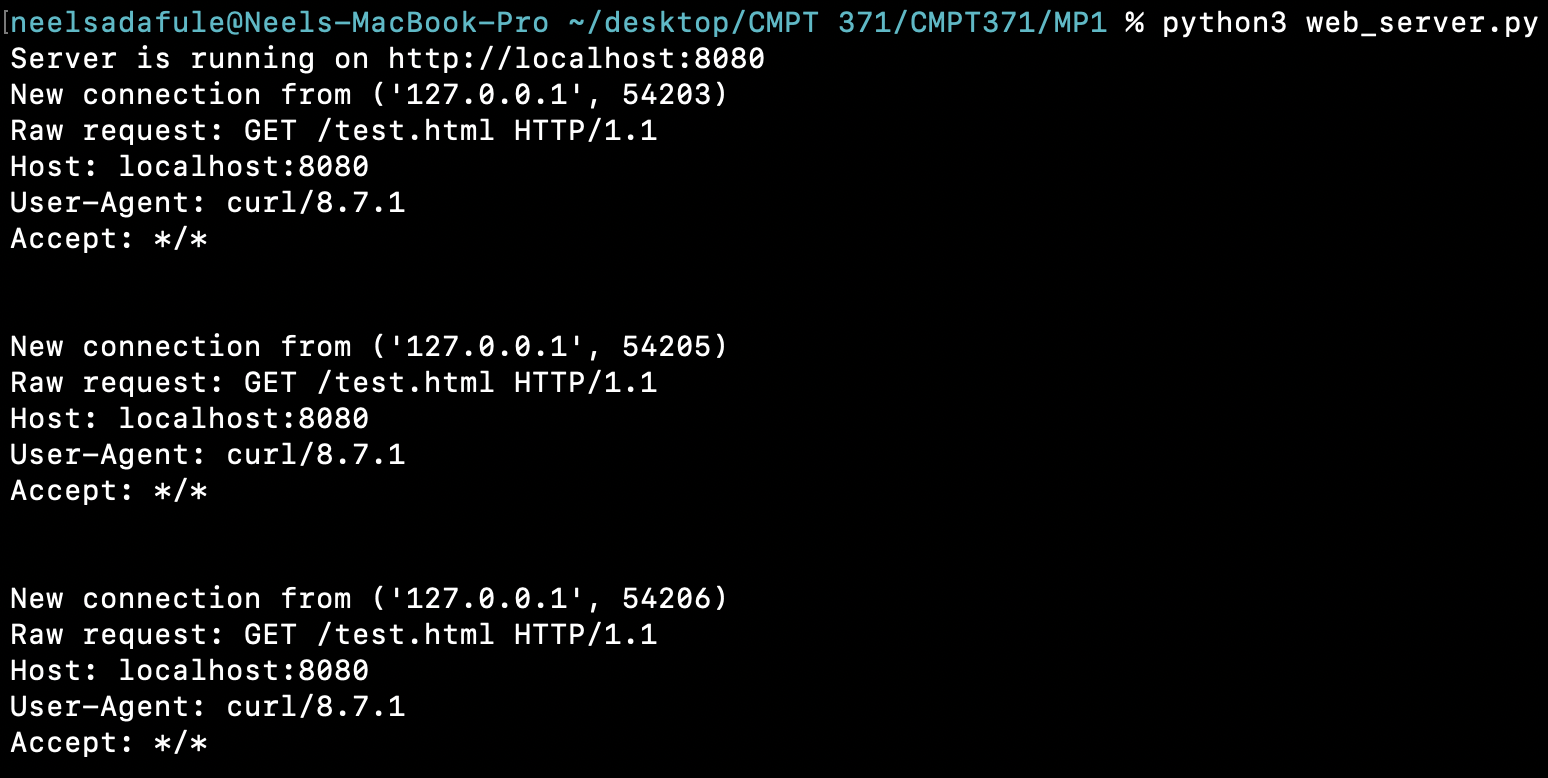
\includegraphics[width=\textwidth]{screenshots/hol_blocking_loop_test_server.png}  % Replace with actual server screenshot
    \end{center}
\end{itemize}

The server successfully handled all 50 concurrent requests, serving content progressively without blocking.

\end{document}
